\section{Optimizers}

\subsection{SGD (Stochastic Gradient Descent)}
Gradyan azalmada tüm veri seti kullanılırken stokastik gradyan azalmada tek bir örneklem kullanılır. Her bir adımda bir örnek seçer ve bu örneğe göre gradyanı hesaplar. Bu yüzden "stokastik" olarak adlandırılır. Küçük veri kümelerinde kullanışlıdır. Tek örnek ile işlem yapıldığı için global minimuma doğru kararlı bir şekilde ilerleme görülmez. Minimaya ulaşmak için daha fazla iterasyon sayısına ihtiyaç duyar.

\begin{figure}[h]
    \centering
    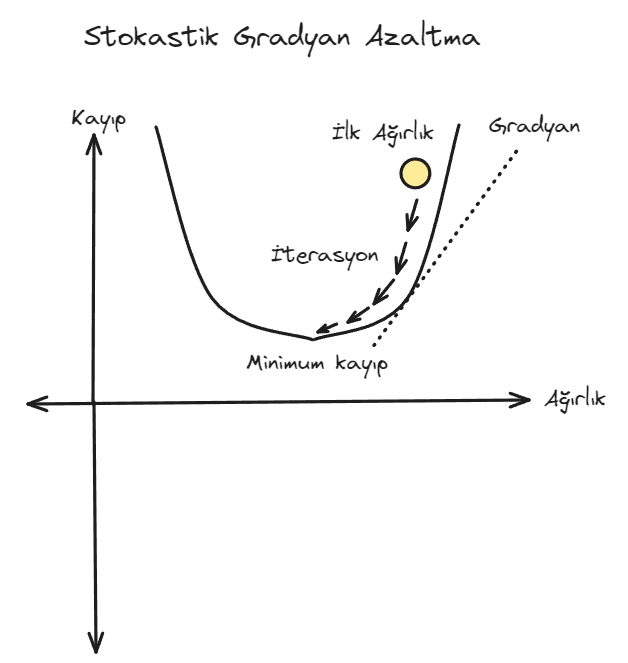
\includegraphics[width=0.7\textwidth]{images/sgd_optimizer.png}
    \caption{SGD optimizasyon algoritması.}
    \label{fig:enter-label}
\end{figure}


\[\theta_{t+1} = \theta_{t} - \alpha \nabla f(\theta_{t})\]
\begin{itemize}
	\item $\theta_(t)$: t zamandaki parametre vektörü
	\item $\alpha$: öğrenme oranı,
	\item $\nabla f(\theta_{t})$: fonksiyonun t zamanındaki gradyanı.
\end{itemize}

\newpage

\subsection{RMSprop (Root Mean Square Propagation)}
Gradyanlara bağlı olarak öğrenme oranını (learning rate) ayarlar. Her parametreyi ayrı ayrı günceller. Eğer bir boyutta gradyanlar büyük ise RMSprop tarafından hesaplanan güncelleme oranı düşer; küçük ise güncelleme oranı artar. Daha az varyans gösteren parametreler daha fazla güncellenir; daha fazla varyans gösteren parametreler daha az güncellenir. Büyük veri setlerinde iyi çalışır.

\begin{figure}[h]
    \centering
    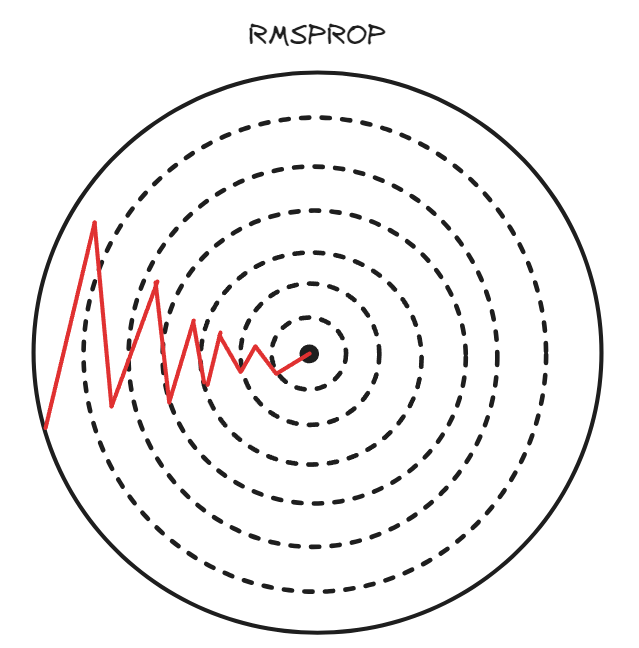
\includegraphics[width=0.7\textwidth]{images/rmsprop_optimizer.png}
    \caption{RMSprop optimizasyon algoritması.}
    \label{fig:enter-label}
\end{figure}

\begin{align*}
E[g^2]_t & = \rho E[g^2]_{t-1} + (1 - \rho) (\nabla f(\theta_t))^2 \\
\theta_{t+1} & = \theta_t - \frac{\alpha}{\sqrt{E[g^2]_t + \epsilon}} \nabla f(\theta_t)
\end{align*}

\begin{itemize}
	\item $\theta_(t)$: t zamanındaki parametre vektörü,
	\item $\nabla f(\theta_{t})$: fonksiyonun t zamanıdaki gradyanı,
	\item $E[g^2]_t$: gradyanların karesinin üstel hareketli ortalaması,
	\item $\rho$: gradyan karesinin üstel azaltma oranı,
	\item $\alpha$: öğrenme oranı,
	\item $\epsilon$: düzeltme terimi.
\end{itemize}

\newpage

\subsection{Adam (Adaptive Moment Estimation)}
Momentum ve RMSprop yöntemlerinin birleşimidir. Birinci ve ikinci momentlerin (hareketli ortalama) eksponensiyel bir şekilde azalan ortalama değerlerini korur ve bu sayede gradyanları güvenilir bir şekilde tahmin eder. Gürültülü veri setleri için uygundur.

\begin{align*}
m_{t+1} & = \beta_{1}m_{t} + (1 - \beta_{1})\nabla f(\theta_{t}) \\
v_{t+1} & = \beta_{2}v_{t} + (1 - \beta_{2})(\nabla f(\theta_{t}))^2 \\
\hat{m}_{t+1} & = \frac{m_{t+1}}{1 - \beta_{1}^{t+1}} \\
\hat{v}_{t+1} & = \frac{v_{t+1}}{1 - \beta_{2}^{t+1}} \\
\theta_{t+1} & = \theta_{t} - \frac{\alpha}{\sqrt{\hat{v}_{t+1}} + \epsilon} \hat{m}_{t+1}
\end{align*}

\begin{itemize}
	\item $\theta_(t)$: t zamanındaki parametre vektörü,
	\item $\nabla f(\theta_{t})$: fonksiyonun t zamanıdaki gradyanı,
	\item $m_{t}$ ve $v_(t)$: t zamanıdaki birinci ve ikinci moment tahminleri,
	\item $\beta_{1}$ ve $\beta_{2}$: momentlerin üstel azalma oranları,
	\item $\hat{m}_{t+1}$ ve $\hat{v}_{t+1}$: düzeltmiş moment tahminleri,
	\item $\alpha$: öğrenme oranı,
	\item $\epsilon$: düzeltme terimi.
\end{itemize}

\newpage

\subsection{AdamW}
Adam yöntemine ağırlık çarpımı (weight decay) eklenmiş bir versiyonudur. Ağırlık çarpımı, modelin karmaşıklığını kontrol etmek ve aşırı uydurmaya karşı koymak için kullanılan bir tekniktir.

\begin{align*}
m_{t+1} & = \beta_{1}m_{t} + (1 - \beta_{1})\nabla f(\theta_{t}) \\
v_{t+1} & = \beta_{2}v_{t} + (1 - \beta_{2})(\nabla f(\theta_{t}))^2 \\
\hat{m}_{t+1} & = \frac{m_{t+1}}{1 - \beta_{1}^{t+1}} \\
\hat{v}_{t+1} & = \frac{v_{t+1}}{1 - \beta_{2}^{t+1}} \\
\theta_{t+1} & = \theta_{t} - \frac{\alpha}{\sqrt{\hat{v}_{t+1}} + \epsilon} \hat{m}_{t+1} - \lambda \theta_{t}
\end{align*}

\begin{itemize}
	\item $\theta_(t)$: t zamanındaki parametre vektörü,
	\item $\nabla f(\theta_{t})$: fonksiyonun t zamanıdaki gradyanı,
	\item $m_{t}$ ve $v_(t)$: t zamanıdaki birinci ve ikinci moment tahminleri,
	\item $\beta_{1}$ ve $\beta_{2}$: momentlerin üstel azalma oranları,
	\item $\hat{m}_{t+1}$ ve $\hat{v}_{t+1}$: düzeltmiş moment tahminleri,
	\item $\alpha$: öğrenme oranı,
	\item $\epsilon$: düzeltme terimi,
	\item $\lambda$: ağırlık bozulma (weight decay) parametresi.
\end{itemize}

\newpage

\subsection{Adadelta}
Parametrelerin güncellenmesi için her adımda değişen bir öğrenme oranı kullanır. Bu oran, parametrelerin hareketli ortalaması ile gradyanın hareketli ortalamasının oranına bağlı olarak hesaplanır. Böylece, büyük gradyanlara küçük, küçük gradyanlarda büyük güncellemeler yapılır.

\begin{align*}
E[g^2]_t & = \rho E[g^2]_{t-1} + (1 - \rho) (\nabla f(\theta_t))^2 \\
\Delta x_t & = - \frac{\sqrt{\Delta \theta_{t-1} + \epsilon}}{\sqrt{E[g^2]_t + \epsilon}} \nabla f(\theta_t) \\
\Delta \theta_t & = \rho \Delta \theta_{t-1} + (1 - \rho) \Delta x_t^2 \\
\theta_{t+1} & = \theta_t + \Delta x_t
\end{align*}

\begin{itemize}
	\item $\theta_(t)$: t zamanındaki parametre vektörü,
	\item $\nabla f(\theta_{t})$: fonksiyonun t zamanıdaki gradyanı,
	\item $E[g^2]_t$: gradyanların karesinin üstel hareketli ortalaması,
	\item $\nabla f(\theta_t)$: parametrelerin karesinin üstel hareketli ortalaması,
	\item $\nabla f(x_t)$: parametre güncellemesi,
	\item $\rho$: gradyan karesinin üstel azaltma oranı,
	\item $\epsilon$: düzeltme terimi.
\end{itemize}

\newpage

\subsection{Adagrad}
Her parametreyi ayrı ayrı güncellerken, daha önceki gradyanların karelerinin toplamını kullanarak öğrenme oranını adapte eder. Daha sık rastlanan gradyan bileşenlerine daha küçük, daha nadir rastlanan gradyan bileşenlerine daha büyük bir öğrenme oranı verilmesini sağlar. Böylece öğrenme oranının manuel olarak ayarlama ihtiyacını kaldırır. Eğitim ilerledikçe, gradyanların karelerinin kümülatif toplamı büyüdükçe, öğrenme oranı küçülür. Bu da eğitim ilerledikçe öğrenme oranının çok hızlı bir şekilde azalmasına neden olabilir.

\begin{align*}
G_{t} & = G_{t-1} + (\nabla f(\theta_t))^2 \\
\theta_{t+1} & = \theta_t - \frac{\alpha}{\sqrt{G_{t} + \epsilon}} \nabla f(\theta_t)
\end{align*}

\begin{itemize}
	\item $\theta_(t)$: t zamanındaki parametre vektörü,
	\item $\nabla f(\theta_{t})$: fonksiyonun t zamanıdaki gradyanı,
	\item $G_{t}$: gradyanların kareleri toplamı,
	\item $\alpha$: öğrenme oranı,
	\item $\epsilon$: düzeltme terimi.
\end{itemize}

\newpage
